\documentclass[10pt,a4paper,titlepage]{article}
\usepackage[latin1]{inputenc}
\usepackage{amsmath}
\usepackage{amsfonts}
\usepackage{amssymb}
\usepackage{graphicx}
\usepackage{listings}
\usepackage{hyperref}
\usepackage[margin=1.00in]{geometry}
\author{Roy Smart \\ Nina (The best dog ever)}
\title{CSCI 476 Computer Security \\ Spring 2015 Final Practicum \\ \texttt{mthack.me} \\ Red Team Penetration Test}



\begin{document}
\maketitle

\tableofcontents

\section{Executive Summary}
In response to an attack on SupraDyne, we performed penetration testing against MHK's network. After gaining access to their network through a variety of means, we were able to find nine flags: mylittlepwnie, DiscoveredIn1655, ThisT1meItsAMoon, TomcatIsAVulnerability, nextlevel, FSInc3ption, deaddrop, logmeinbro, and haxtheplanet. These flags demonstrated that MHK's network has some severe vulnerabilities that need to be addressed.

To locate these flags we used a variety of exploits and tools. Google Chrome was used to analyze websites and parse HTML code. Nmap was used to scan web servers and locate vulnerable services. Metasploit modules were used to brute force Tomcat default credentials. Laudanum was used to exploit Tomcat servers and gain access to root shells. Radare2 was utilized to reverse executable binaries and determine the information hidden within. To recover files we used the program Testdisk on various disk images, and used Fcrackzip to extract password-protected archives contained in the images.

Considering that tools readily available on the internet were used to infiltrate MHK's organization, we would rate the risk for this organization fairly high. While there were certainly some servers that we could not gain penetrate, the extent of our access was certainly troubling to say the least.
\section{Narrative}
It came to our knowledge that our company (SupraDyne) had been attacked by Germany's infamous MtHack Krew (MHK) and sensitive data may have been compromised. In retaliation, we were authorized by the Department of Defense to initiate a counterattack. To start this attack, we were provided some intelligence on MHK along with possible attack vectors\cite{test}. The penetration testing undertaken was divided into separate rounds, with each round attacking a particular section of the MHK organization. Recovered data is represented as flags, denoted in the format \texttt{flag:this\_is\_a\_flag}.
\subsection{Round 1}
For this round, we were provided with the URL of MHK's main website: \url{http://mthack.me}. Intelligence\cite{test} also informed us that there were three potential flags hidden within the website.
\subsubsection{Flag: My Little Pwnie}
To begin, we navigated to MHK's website to gather some more information. \\
\begin{center}
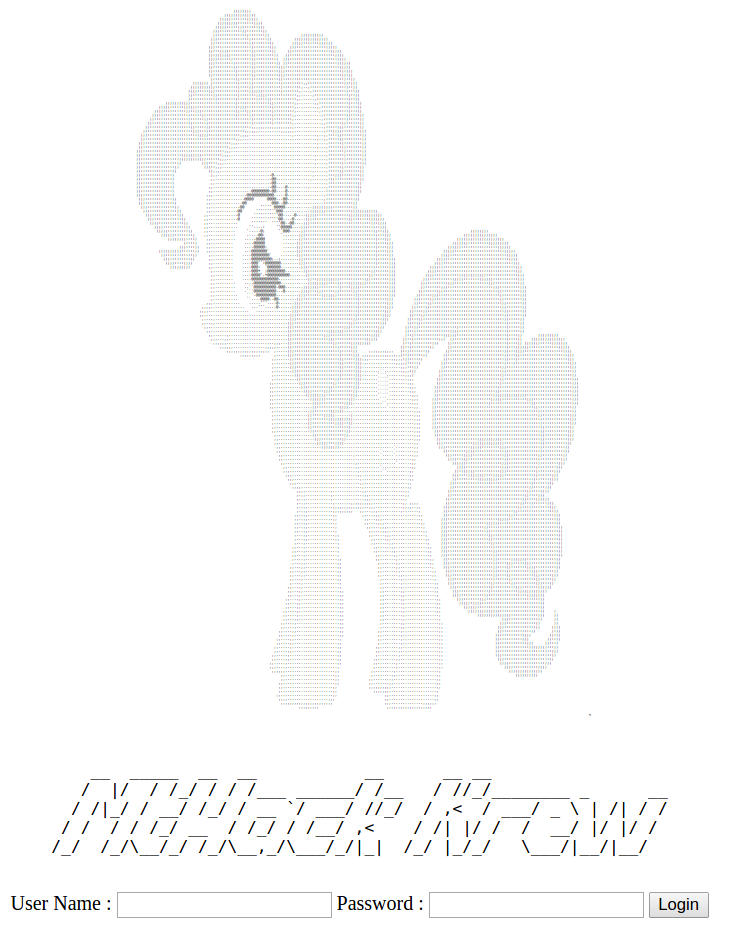
\includegraphics[width=0.4\textwidth]{mthack_flags/mylittlepwnie/web}
\end{center}
The User Name and Password fields to access the site looked interesting, so we took a look at the HTML source to find out more. \\
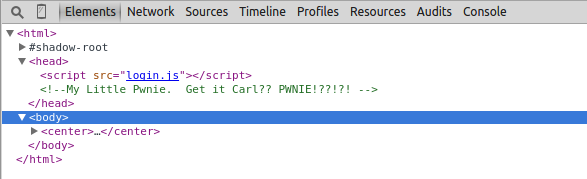
\includegraphics[width=0.49\textwidth]{mthack_flags/mylittlepwnie/source}
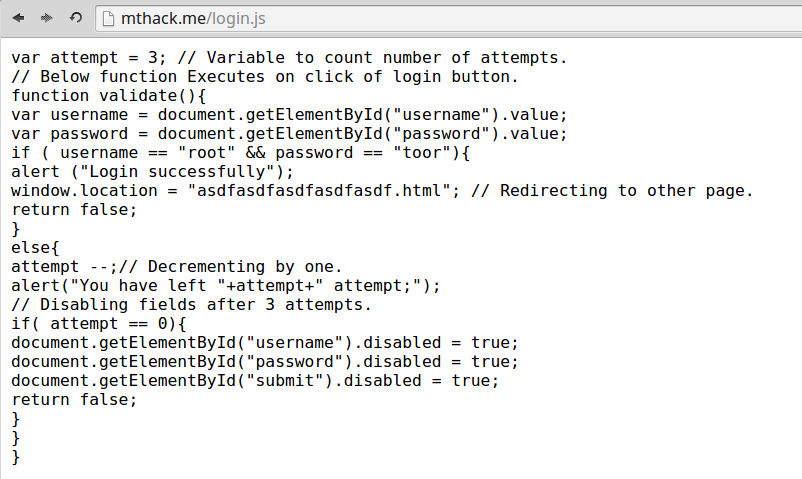
\includegraphics[width=0.49\textwidth]{mthack_flags/mylittlepwnie/js} \\
Within the source, we found a reference to a Javascript file that looked interesting, \texttt{login.js}. After navigating to the script in our web browser, we found that the script contained some very vulnerable information: a valid username (\texttt{root}) and password (\texttt{toor}), along with details concerning how the website validates users. After logging in with the new username and password, we were presented with a webpage that contained the flag.
\begin{center}
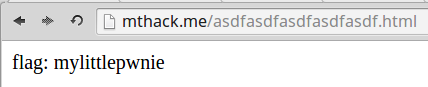
\includegraphics[width=0.5\textwidth]{mthack_flags/mylittlepwnie/flag}
\end{center}
\subsubsection{Determining Subdomains of \texttt{mthack.me}}
In the provided intelligence\cite{test}, there were references to MHK members joking about something known as ``rfc 2100". A little research determined that this referred to a poem by J. Ashworth titled ``The Naming of Hosts" \cite{rfc}. Enumerated in the poem are several hypothetical hostnames for servers. We constructed a dictionary out of all of the words contained in the poem to attempt to brute force subdomains of \texttt{mthack.me}. Using the program \texttt{dnsenum} provided in Kali Linux, we were able to identify four additional subdomains of \texttt{mthack.me}:
\begin{itemize}
\item \texttt{hobbes.mthack.me}
\item \texttt{sirius.mthack.me}
\item \texttt{titan.mthack.me}
\item \texttt{europa.mthack.me}
\end{itemize}
These subdomains provided additional attack vectors through which we could gain access to MHK's network.
\subsubsection{Flag: Discovered in 1655}
To probe further into the MHK organization, we decided to mount attack against the subdomain \texttt{titan.mthack.me}. Using the program \texttt{nmap}, we executed a fast SYN stealth port scan against the subdomain. 
\[ \texttt{sudo nmap -sS -T4 -v -F titan.mthack.me -Pn} \]
This port scan revealed that port 23 was open for business. A quick internet search revealed that port 23 is often used as a telnet port. Armed with this information, we launched the program \texttt{telnet} against \texttt{titan.mthack.me} and found a flag in the banner message provided by the server's telnet client.
\begin{center}
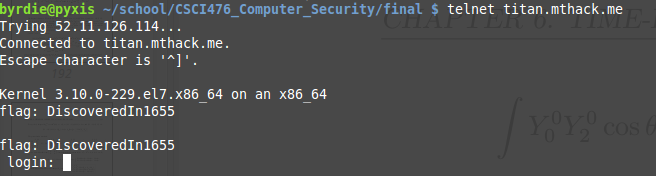
\includegraphics[width=0.5\textwidth]{titan_flags/DiscoveredIn1655/flag}
\end{center}
\subsubsection{Flag: This T1m3 its a Moon}
Further fast \texttt{nmap} scans against the other domains did not provide any new information. So in search of a new service to attack, we performed a full port scan against the subdomain \texttt{europa.mthack.me} using \texttt{nmap}.
\begin{center}
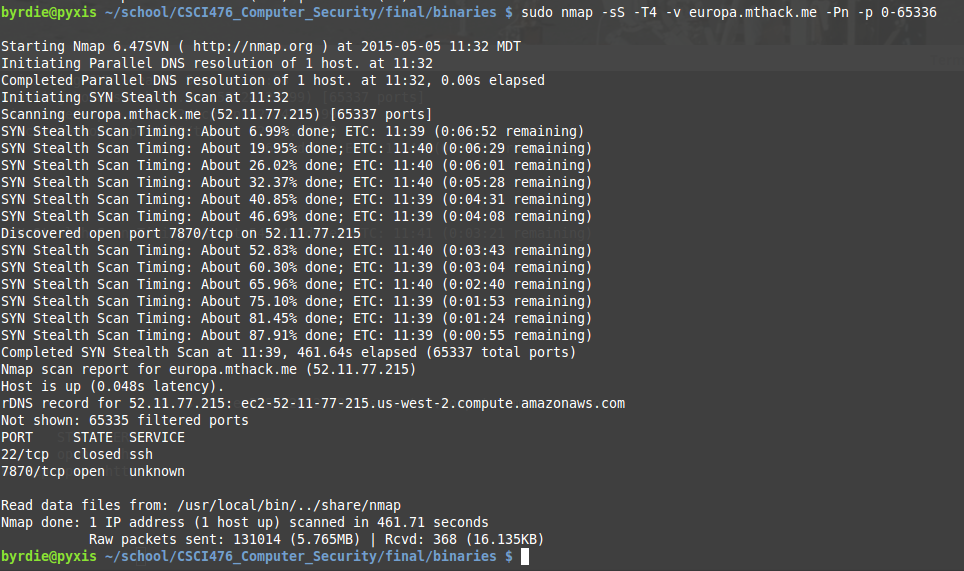
\includegraphics[width=0.5\textwidth]{europa_flags/Th1sTi1m3ItsAMoon/nmap}
\end{center}
The full port scan revealed an unknown service on port 7870. Using the program \texttt{netcat} against that port revealed that there was an SSH server operating on that port. Opening an \texttt{ssh} session on that port revealed the flag in the banner message provided by the SSH server.
\begin{center}
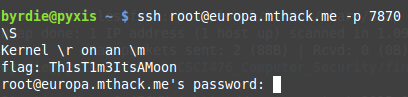
\includegraphics[width=0.5\textwidth]{europa_flags/Th1sTi1m3ItsAMoon/flag}
\end{center}
\subsection{Round 2}
For round 2, intelligence \cite{test} provided an additional subdomain of MHK's network: \texttt{mercury.mthack.me}. Intelligence also informed us that there was one flag hidden in the server.
\subsubsection{Flag: Tomcat is a Vulnerability}
A fast \texttt{nmap} port scan informed us that there was a service operating on port 8089 of \texttt{mercury.mthack.me}. An internet search reported that this port is used by the Tomcat web server. Navigating to the site in our browser showed us the default Tomcat page.
\begin{center}
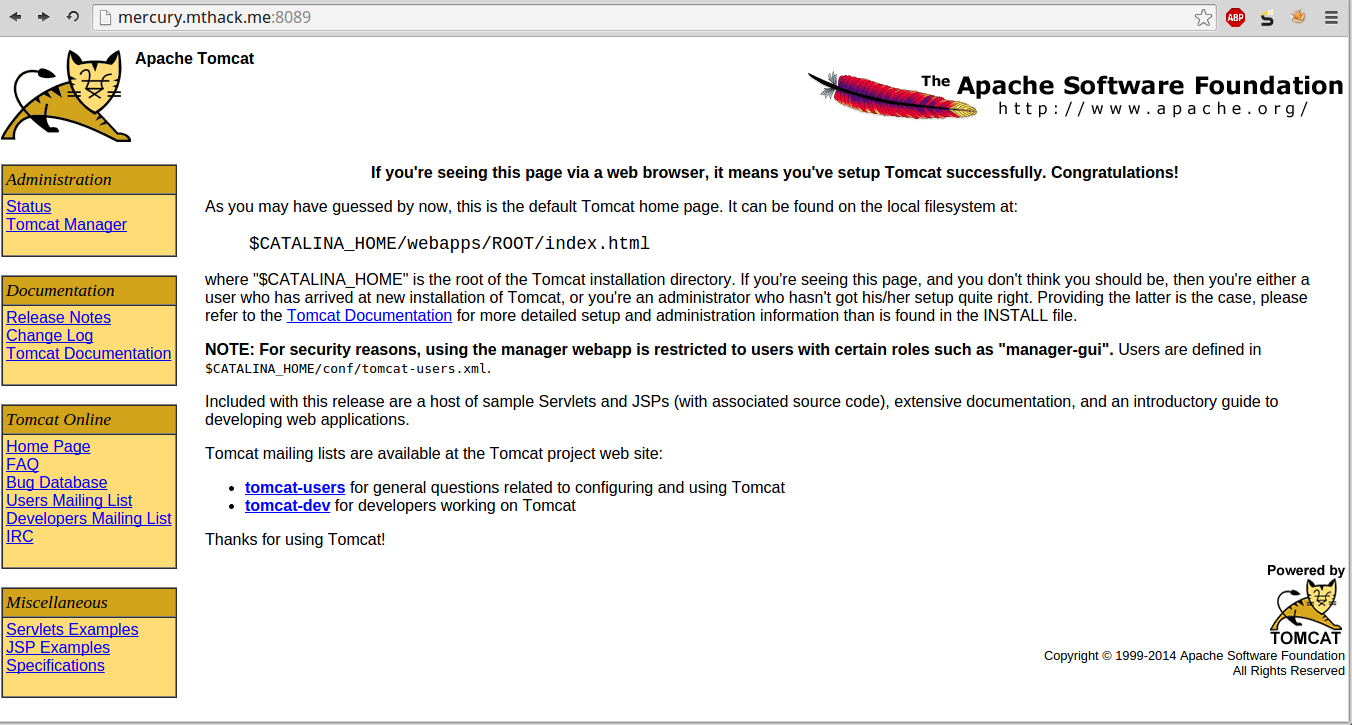
\includegraphics[width=0.5\textwidth]{mercury_flags/TomcatIsAVulnerability/tomcat}
\end{center}
A quick search for flags hidden on this page was unsuccessful, and the only interesting links appeared to be the \texttt{Status} and \texttt{Tomcat Manager} links on the upper right hand corner of the page. Unfortunately these links were password protected and we had not been provided any clues towards a possible username and password. To solve this problem we turned to the Metasploit plugin \texttt{tomcat\_mgr\_login}. This program provided a dictionary of default usernames and passwords used for Tomcat installations and had the ability to brute force an instance of Tomcat until the credentials were found. After a short run, the plugin revealed the username (\texttt{tomcat}) and the password \texttt{tomcat}.
\begin{center}
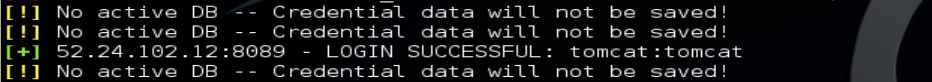
\includegraphics[width=0.5\textwidth]{mercury_flags/TomcatIsAVulnerability/found}
\end{center}
With the user credentials in hand, we were able to explore the \texttt{status} section of the server. While this did not give us access to the site, we did notice a section that gave us the ability to upload \texttt{WAR} files. Following a tutorial written by Tony Lee \cite{tomcat}, a method to upload a shell exploit was determined. Using a \texttt{WAR} file included in the Laudanum project \cite{Laudanum}, we were able to upload it to the server and gain access to a root shell.
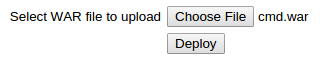
\includegraphics[width=0.5\textwidth]{mercury_flags/TomcatIsAVulnerability/war}
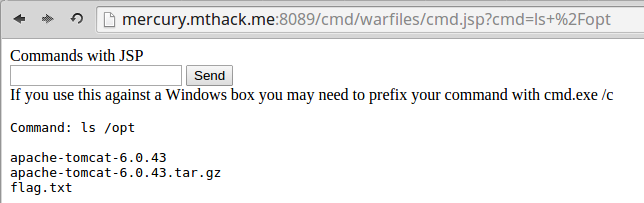
\includegraphics[width=0.5\textwidth]{mercury_flags/TomcatIsAVulnerability/cmd} \\
Through poking around the directories, we were able to find root's \texttt{.bash\_history} file. We found that the last person to use the root account opened the \texttt{/opt/} directory and placed a file named \texttt{flag.txt} into the directory. Using the program \texttt{cat} within our shell exploit, we were able to read the flag's contents.
\begin{center}
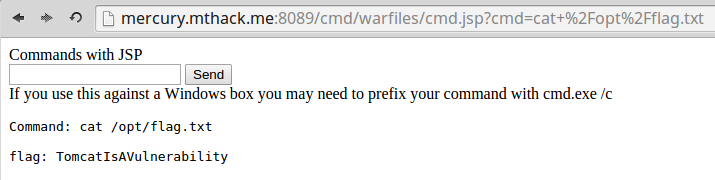
\includegraphics[width=0.5\textwidth]{mercury_flags/TomcatIsAVulnerability/flag}
\end{center}
\subsection{Round 3}
For this round, prior intelligence was able to recover an executable binary used to test new hacking recruits. The number of known flags contained within the binary was unspecified.
\subsubsection{Flag: Next Level}
To reverse the provided binary, we used the program \texttt{radare2}. This program allows the compiled assembly code to be more human readable. Running the command \texttt{pd@sym.main} allowed us to look at the main function of the binary.
\begin{center}
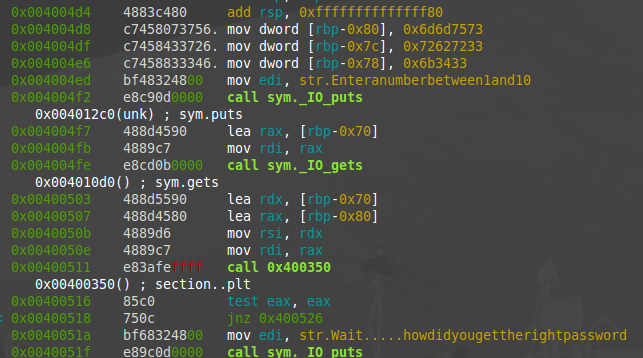
\includegraphics[width=0.5\textwidth]{binary_flags/nextlevel/radare2}
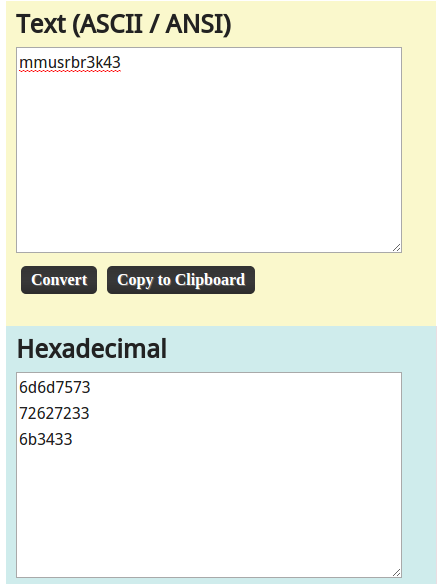
\includegraphics[width=0.3\textwidth]{binary_flags/nextlevel/hex_to_ascii}
\end{center}
Near the top of \texttt{radare2}'s output above, we can see that several hexadecimal values are pushed onto the stack. We correctly guess that these hex values contain the \texttt{ascii} representation of the password. We used a web service to convert the hexadecimal representation to an \texttt{ascii} representation.
Unfortunately the password has an endianess problem. Since the values are pushed onto the stack in reverse order, we need to flip each 32-bit hex value (or each set of four characters). Doing this gives us the correct password \texttt{summ3rbr34k}. With the correct password in hand, we are free to run the provided binary to see what we find.
\begin{center}
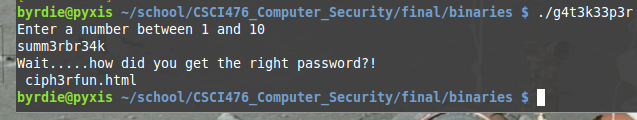
\includegraphics[width=0.49\textwidth]{binary_flags/nextlevel/output}
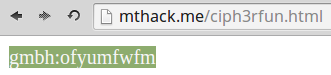
\includegraphics[width=0.40\textwidth]{binary_flags/nextlevel/cipher}
\end{center}
The output of the program provides an html file, which we correctly assumed was a subdirectory of \texttt{mthack.me}. Navigating our browser to the appropriate page supplies some text that looks very similar to the format of previous flags, however it appears to be encrypted using a Cesarean cipher. Using a web service \cite{ceasar} to apply a Cesarean shift of 25 to the above text reveals the flag.
\begin{center}
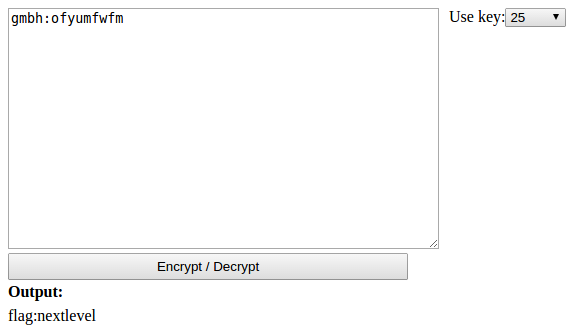
\includegraphics[width=0.49\textwidth]{binary_flags/nextlevel/ceasar}
\end{center} 
\subsection{Round 4}
Again for round 4, previous intelligence was able to locate important files used by the MHK organization. In this case the data was an image of a 50 MB drive. We are told that it contained two flags. Opening the drive with the program \texttt{testdisk} allowed us to recover two files.
\begin{center}
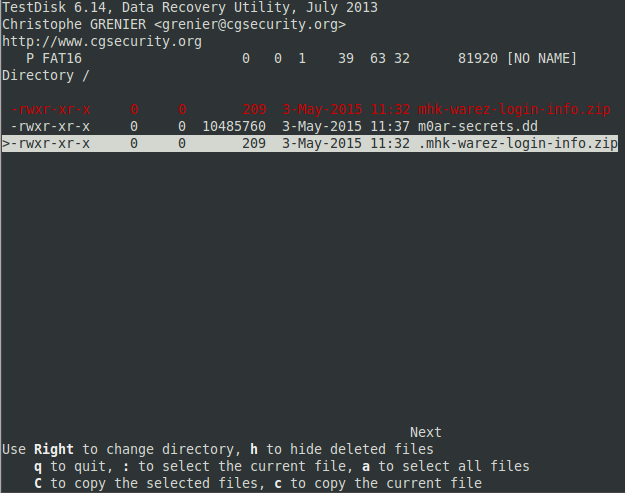
\includegraphics[width=0.3\textwidth]{zip_flags/testdisk}
\end{center}
\subsubsection{Flag: FS Inc3ption}
Within the files recovered from the 50 MB disk image, there appeared to be another disk image, labeled \texttt{m0ar-secrets.dd}. Running \texttt{strings} through the filter program \texttt{grep} revealed the flag.
\begin{center}
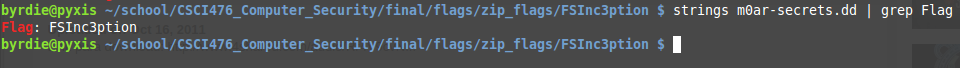
\includegraphics[width=0.7\textwidth]{zip_flags/FSInc3ption/flag2}
\end{center}
\subsubsection{Flag: Deaddrop}
Also contained within the 50 MB disk image was a file \texttt{mhk-warez-login-info.zip} archive. Attempting to extract this archive showed us that it was encrypted with a password. We used a program provided by Kali called \texttt{fcrackzip} to brute force the password. Since the program is fairly light, we were able to use the ubiquitous \texttt{rockyou.txt} wordlist to quickly find the password: \texttt{blessed}.
\begin{center}
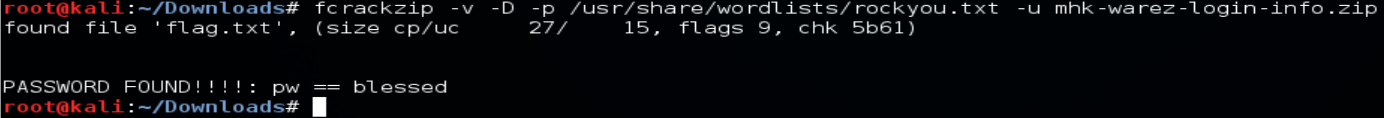
\includegraphics[width=0.7\textwidth]{zip_flags/deaddrop/fcrack}
\end{center}
With the password, we were able to extract the archive and find the file named \texttt{flag.txt}. The contents of the file were \texttt{Flag:deaddrop}.
\subsection{Round 5}
For round 5, a field agent was able to get close to MHK's base of operations and acquire a packet capture of wireless traffic on their network. We were informed that there were three potential flags hidden in the packet capture.
\subsubsection{Flag: Log Me in Bro}
To find this first flag, we to simply ran \texttt{strings} with the \texttt{grep} filter ``Basic".
\begin{center}
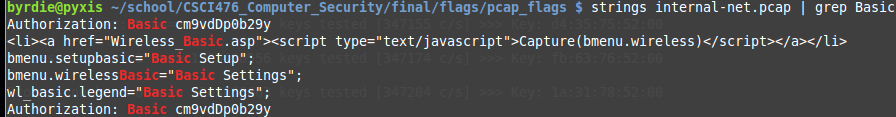
\includegraphics[width=0.65\textwidth]{pcap_flags/logmeinbro/basic}
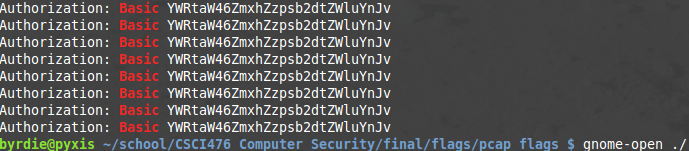
\includegraphics[width=0.5\textwidth]{pcap_flags/logmeinbro/base64}
\end{center}
The output revealed a \texttt{base64} number that was converted to find the flag.
\begin{center}
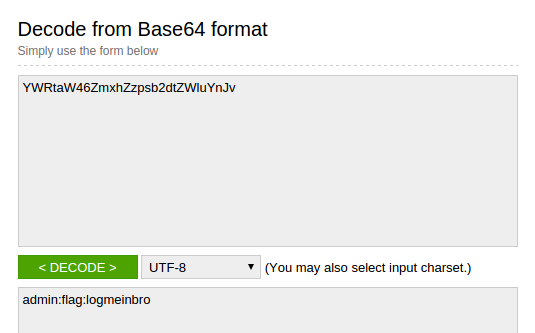
\includegraphics[width=0.5\textwidth]{pcap_flags/logmeinbro/flag}
\end{center}
\subsubsection{Flag: Hax the Planet}
To make things difficult, the capture included packets encrypted with WEP. We used \texttt{airdecap-ng} to partially decrypt the packet capture.
\begin{center}
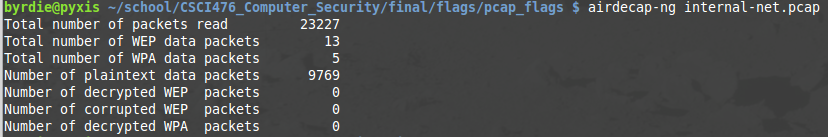
\includegraphics[width=0.5\textwidth]{pcap_flags/haxtheplanet/decap}
\end{center}
After this was complete, we simply ran \texttt{strings} with the filter ``flag" to find the final flag.
\begin{center}
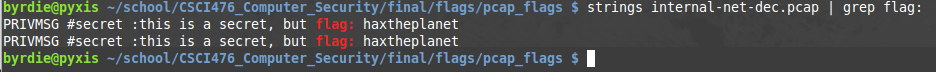
\includegraphics[width=0.5\textwidth]{pcap_flags/haxtheplanet/flag}
\end{center}
\section{Summary}
Using Kali Linux and a variety of tools available on the internet, MHK's organization was successfully compromised and a number of flags were identified. Some servers such as Sirius and Hobbes were unaccessible to us, so at least some of MHK's servers would remain safe in the event of a real attack.

We recommend that MHK takes some serious steps to beef up security. This includes: updating their main site \texttt{mthack.me} with a more robust credential system; changing their Tomcat user name and password from the default setting and preferably not using Tomcat all together; and finally, using passwords which are not words, e.g. those which would not appear in wordlists such as Rockyou.

We would like to thank the Department of Defense, SupraDyne, and MHK for allowing us to conduct this penetration test. We hope that those organizations will come to us if they need any more work done on this subject.
\bibliographystyle{unsrt}
\bibliography{sources}

\end{document}